% !TEX root =../LibroTipoETSI.tex
\chapter{PF\_RING}\LABCHAP{PFRING}
\pagestyle{esitscCD}

\epigraph{In almost every computation a great variety of arrangements for the succession of the processes is possible, 
and various considerations must influence the selections amongst them for the purposes of a calculating engine. One 
essential object is to choose that arrangement which shall tend to reduce to a minimum the time necessary for completing 
the calculation.}{Ada Lovelace}

%\lettrine[lraise=0.7, lines=1, loversize=-0.25]{E}{l} 
\lettrine[lraise=-0.1, lines=2, loversize=0.25]{E}n un sistema de monitorización de tráfico, la captura de paquetes es 
un proceso vital. Si se quiere capturar tráfico a una velocidad aceptable, superiores a 1Gbps, es necesario que todo el 
proceso de captura de paquetes esté bien diseñado y sea eficiente. De no serlo, enseguida comenzaremos a notar 
pérdidas de paquetes, y nuestra monitorización no será efectiva.

%TODO unir con lo demás
Ya hemos cubierto la eficiencia en términos de procesamiento de paquetes en los anteriores capítulos. 

\gls{PFRING} es, según su autor Luca Deri, una tecnología que persigue capturar tráfico a $10G$ sin necesitar tarjetas 
especializadas, sin pérdidas y bajo cualquier circunstancia del tráfico, de forma que sea posible crear sondas de 
tráfico software con el mismo rendimiento que las basadas en hardware \cite{LucaDeriPFRING}.

A lo largo de este capítulo, %TODO

\section{Conceptos preliminares}
\subsection{Interrupción}
\subsection{Programador de tareas}
\subsection{Llamada al sistema}
\subsection{Memoria mapeada o mapeo de memoria}

\section{Proceso de paquetes por el núcleo linux}\LABSEC{sec:ProcesoPaquetesLinux}
El paso de paquetes a través del núcleo Linux puede ser un importante cuello de botella. %TODO ampliar

\subsection{Reserva de memoria para almacenar el paquete}
El primer paso en la recepción de paquetes es que éste llegue a la tarjeta de red a través de la interfaz física. Tan 
pronto como esto ocurre, y la memoria interna de la \gls{NIC} contiene el paquete completo, ésta es responsable de 
de crear una estructura de datos para almacenar el paquete en la memoria principal del sistema, y copiarlo ahí.

Esta reserva ya incluye un corte en términos de tiempo, ya que dos procesos no pueden reservar memoria al mismo tiempo. 
El sistema tiene una tabla de memoria en la que están anotados los distintos bloques que cada proceso (incluído el 
núcleo) tiene reservada. Si dos procesos reservasen al mismo tiempo, podría ocurrir que reservasen segmentos de memoria 
solapados.

Por tanto, la reserva debe ser sincronizada, y esta sincronización consume un tiempo importante. Tras ello, la copia es 
en modo \gls{DMA}, por lo que la tarjeta obtiene acceso exclusivo a esa memoria y no es necesario la intervención de la 
CPU para copiar los datos.

El paquete es entonces copiado en una estructura de datos \texttt{sk\_buff}. Dicha estructura es bastante grande, y 
puede ir creciendo a medida que lo necesita. Esto incrementa la fragmentación de memoria, ya que al crecer es posible 
que no quepa en su segmento de memoria, y deba moverse a otro segmento mayor.

Por último, existen bastantes datos de la estructura que son privados, y no deben viajar de una capa a otra en el paso 
de información. Por tanto, hay que clonar la estructura al transmitir información\footnote{Si bien hay partes de la 
misma que pueden mantenerse}, lo que redunda en más reservas y más retrasos por sincronía
\cite{skBuffLinuxFoundation}.

\subsection{Notificación del nuevo paquete}
Cuando el paquete al completo es copiado en la memoria principal, es necesario un mecanismo de notificación al 
\gls{controlador}\index{Controlador de Dispositivo} de red de Linux para que éste pueda procesarlo. Se usa, entonces, 
una interrupción hardware.

La interrupción provoca que el núcleo deje de realizar las tareas que esté haciendo para hacer caso a la llegada del 
paquete. Sin embargo, si tenemos demasiados paquetes por segundo, no dejamos a Linux avanzar, y destrozamos la 
planificación de tareas. Este hecho es conocido como Tormenta de Interrupciones\index{Tormenta de Interrupciones} o 
\emph{interrupt storm} \cite{p206}.

En cada interrupción, la función llamada es \texttt{netif\_rx}.

\subsubsection{NAPI}
Para evitar la tormenta de interrupciones, se pueden utilizar técnicas como la llamada \emph{device polling}. El 
funcionamiento es el siguiente \cite{beyondDevicePolling}.
\begin{itemize}
 \item Cuando un nuevo paquete llega, la tarjeta genera una interrupción.
 \item El \gls{SO} la maneja de la siguiente forma:
 \begin{enumerate}
  \item Prohíbe (enmascara) futuras interrupciones del dispositivo.
  \item Programa una tarea para atender a la tajeta en un futuro.
  \item Cuando la atiende, levanta la prohibición de interrupciones.
 \end{enumerate}
\end{itemize}

La implementación de esta técnica en Linux es conocida como \gls{NAPI}.

Podemos ver en las figuras \FIG{InterrupcionesNIC} y \FIG{DevicePolling} las diferencias entre un canal saturado 
con un método y otro. Se observa como, en la primera figura, al núcleo no le da tiempo a procesar todos los paquetes 
del canal saturado, y sólo puede procesar una de cada dos. Sin embargo, en la segunda figura, Linux procesa los 
paquetes cuando puede, en tiempos aleatorios, y coge de una tacada todos los paquetes que necesita.

\begin{figure}[hbtp]
\centering
%\hfill
\subfloat[Interrupción]%
   {\LABFIG{InterrupcionesNIC}%
   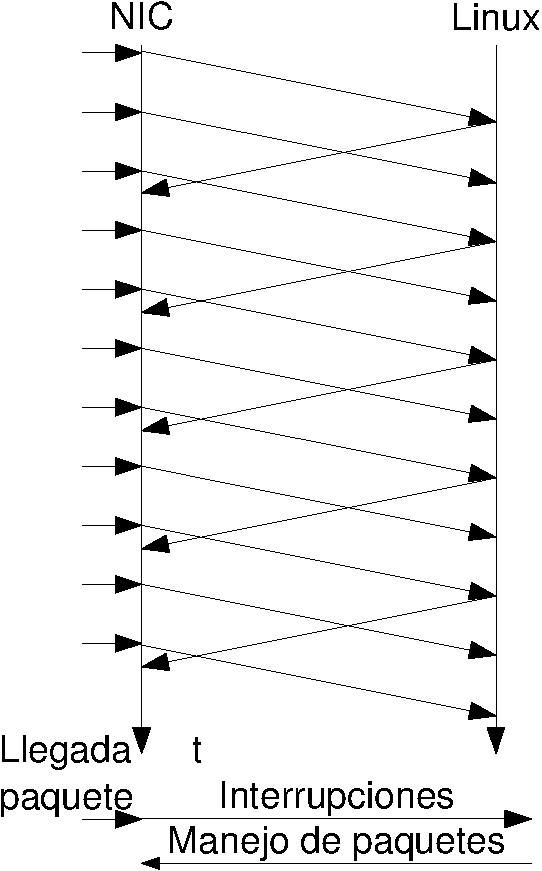
\includegraphics[width=0.30\textwidth]{CapituloPF_RING/Figuras/InterrupcionesNIC-crop}}%
\hspace{0.2\textwidth}
\subfloat[Device Polling]%
 {\LABFIG{DevicePolling}%
 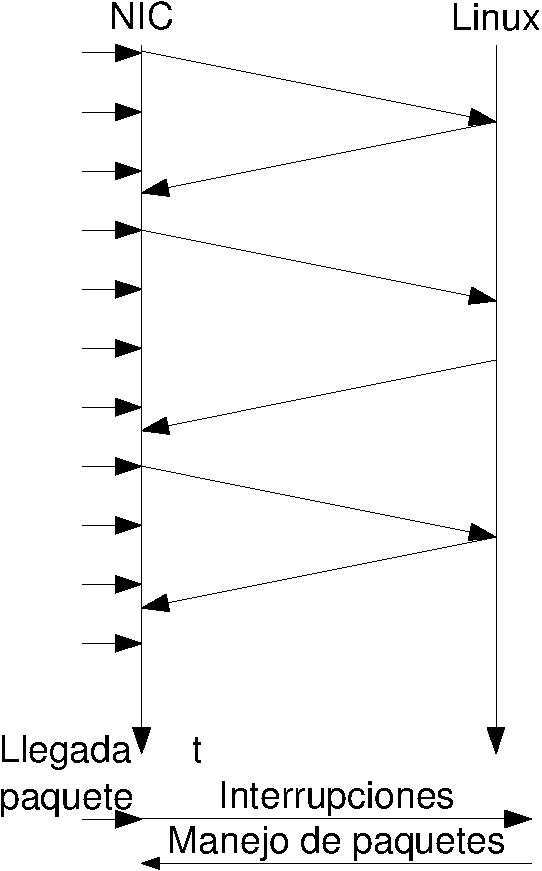
\includegraphics[width=0.30\textwidth]{CapituloPF_RING/Figuras/PollNIC-crop}}%
%
\caption{Comparativa entre los diferentes métodos de notificación de nuevos paquetes}
\end{figure}
%

Si se quiere usar NAPI, la función usada para traer paquetes es \texttt{netif\_receive\_skb}.

\subsection{Obtención del paquete por parte del kernel}
Una interrupción debe ser rápida, esto es, en una interrupción no podemos realizar tareas que no sean estrictamente 
necesarias, por las mismas razones que las señales en espacio de usuario. Por ello, la interrupción provoca que se 
planee una tarea con el fin de recoger el paquete.

A partir de ese momento, sólo cuando el planeador decida que el sistema está libre, se recogerá el / los paquetes 
usando \texttt{packet\_rcv}, y se pasará a la pila de red de Linux.

En la pila, el paquete pasará por diversos sistemas, como la parte de filtrado 
\emph{\gls{netfilter}}\index{Netfilter} para, finalmente, ser recibido por un puerto o \emph{\gls{socket}} llegar a 
estar listo para la recogida por parte del espacio de usuario \cite{p206}.

\subsection{Obtención del paquete por parte del espacio de usuario}
La recepción de paquetes en el espacio de usuario se realiza mediante la librería \emph{\gls{libpcap}}\index{libpcap}.
Para ello, \emph{\gls{libpcap}} genera un \emph{\gls{socket}} que es abstraído por un descriptor de fichero. 

La llamada al sistema \texttt{read}, y su envoltorio para \emph{sockets} \texttt{readfrom}, sirve para leer datos 
que el núcleo le pasa. Sin embargo, esta llamada es bloqueante, el hilo estará bloqueado hasta que se reciban datos por 
lo que no podremos procesar otro tipo de señales o eventos.

Por ello, existe otra llamada al sistema \texttt{select} o \texttt{poll}. Con ellas, el hilo duerme un determinado 
número de milisegundos, pero despierta si el \emph{\gls{socket}} queda listo para lectura. De esta forma, sólo 
llamaremos a \texttt{read} si es necesario, y no congelaremos el hilo.

Es importante no confundir el \texttt{poll} del espacio de usuario con el \emph{device polling}. Pese a que los 
conceptos son similares, el primero lo realiza un proceso de usuario hacia el núcleo, y el segundo lo realiza el núcleo 
hacia el dispositivo de red.

\begin{lstlisting}[language=C++,caption={Lectura desde un socket crudo}, 
breaklines=true, label=code:lecturaRawSocket,numbers=left,float=phtb]
#include<stdio.h>
#include<string.h>

#include<net/ethernet.h>
#include<sys/socket.h>
#include<arpa/inet.h>
#include<sys/ioctl.h>
#include<sys/types.h>
 
void ProcessPacket(char* , int);
 
int main(){
    size_t saddr_size, data_size;
    struct sockaddr saddr;
         
    char buffer[65536];
   
    int sock_raw = socket(AF_PACKET, SOCK_RAW, htons(ETH_P_ALL));
    setsockopt(sock_raw, SOL_SOCKET, SO_BINDTODEVICE, "eth0", 
                                               strlen("eth0")+1);
     
    if(sock_raw < 0){
        perror("Socket Error");
        return 1;
    }
    while(1){
        struct pollfd fds = { fd: sock_raw, events: POLLIN};
        const int poll_rc = poll(&fsd, 1, 1000);
        if(poll_rc == 0){
            if(poll_rc <= 0)
                perror("Poll error");
            continue;
        }
        saddr_size = sizeof(saddr);
        //Receive a packet
        data_size = recvfrom(sock_raw, buffer, 65536, 0, &saddr, 
                                       (socklen_t*)&saddr_size);
        if(data_size < 0){
            printf("Recvfrom error , failed to get packets\n");
            return 1;
        }
        //Now process the packet
        ProcessPacket(buffer , data_size);
    }
    close(sock_raw);
    return 0;
}
\end{lstlisting}

Un ejemplo de este tipo de lecturas podemos verlo en en \lstlistingname{} \ref{code:lecturaRawSocket}. En él, vemos la 
creación del socket con \texttt{socket}, la consulta de disponibilidad con \texttt{poll} y la recepción de los datos 
con \texttt{recvfrom}.

Sin embargo, este procedimiento tiene un coste oculto. A la hora de leer los datos, estos son copiados desde la 
memoria del núcleo a un buffer en espacio de usuario. Esto es, por cada paquete, estamos perdiendo tiempo y ciclos de 
CPU en copiar un dato que sólo vamos a leer.

Si, por ejemplo, queremos leer paquetes de 150kb en un enlace saturado a una velocidad de 1Gbps, estamos realizando:
\begin{itemize}
 \item $\frac{1G}{150k} \approx 7000$ llamadas al sistema con \texttt{poll} y otras tantas con \texttt{recvfrom}.
 \item Copiando entre regiones de memoria RAM a 1Gbps.
\end{itemize}

Resumiendo, por cada paquete recibido, tenemos:
\begin{enumerate}
 \item Reserva de memoria, con pérdidas por sincronización.
 \item Copia de memoria a la estructura reservada.
 \item Potencial interrupción del núcleo.
 \item Espera a la lectura del paquete, ya que ésta se programa.
 \item Llamada al sistema para conocer si el socket está listo
 \item Copia de memoria al espacio de usuario.
\end{enumerate}

\section{La alternativa: PF\_RING}\LABSEC{La alternativa: PF RING}
Luca Deri propuso crear un camino directo desde la tarjeta de red hasta el espacio de usuario, que evitase realizar 
todas las operaciones ineficientes que Linux necesita. % TODO: ampliar

\subsection{Buffer circular}
Para ello \cite{beyondDevicePolling}:

\begin{itemize}
  \item Se crea un nuevo tipo de socket \texttt{PF\_RING}, orientado a la captura pasiva de paquetes. Se basará 
en un buffer circular, donde los paquetes se copian a medida que llegan al sistema
  \item El anillo es reservado a la creación del socket, y liberado a la finalización. Sockets diferentes tendrán 
anillos diferentes.
  \item Los paquetes no serán enviados a la pila del núcleo por defecto, de manera que este nuevo socket no sea una 
sobrecarga sino un camino alternativo.
  \item Los paquetes serán accesibles desde el espacio de usuario vía mapeado de memoria o \texttt{mmap}\index{mmap}, 
eliminando así la copia de memoria entre el espacio del núcleo y el espacio de usuario.
  \item Se crea un hilo en el núcleo específico para obtener paquetes, por lo que no afectará tanto la programación de 
la recepción.
  \item Cuando llegan paquetes, y son copiados en el anillo, Linux desplaza hacia delante el puntero de escritura. 
Cuando son leídos del anillo, se desplaza hacia delante el puntero de lectura.
  \item Nuevos paquetes sobre-escriben paquetes antiguos. Si el anillo está lleno, los paquetes son descartados.
\end{itemize}

Como resultado, Luca Deri sigue registrando pérdidas, y observa que son debidas a la llamada \texttt{poll} de espacio 
de usuario. En ella, aunque haya paquetes esperando, se desperdician muchos ciclos de CPU. Por ello, se pregunta, antes 
de realizar la llamada, si existen paquetes en el anillo (espera activa). Si la respuesta es no, se realiza la llamada 
a \texttt{poll}.

\begin{lstlisting}[language=C++,caption={Lectura de paquetes con poll en el núcleo}, 
breaklines=true, label=code:PFRINGKernelPoll,numbers=left,float=htbp]
sockFd = socket(PF_RING, SOCK_RAW, htons(ETH_P_ALL);
   ..
ringBufferPtr = mmap(NULL, ringSize,
                     PROT_READ|PROT_WRITE,MAP_SHARED, sockFd, 0);
slotId = &ringBufferPtr->slotId;

while(1) {
    if(ringBufferPtr->slot [slotId].isFull) {
        readPacket(ringBufferPtr->slot [slotId]);
        ringBufferPtr->slot [slotId].isFull = 0;
        slotId = (slotId + 1) % ringSize;
    } else {
        /* Sleep when nothing happens */
        pfd.fd = fd;
        pfd.events = POLLIN|POLLERR;
        pfd.revents = 0;
        poll(&pfd, 1, -1);
    }
}
\end{lstlisting}

\begin{lstlisting}[language=C++,caption={Lectura de paquetes con poll en el espacio de usuario}, 
breaklines=true, label=code:PFRINGUserspacePoll,numbers=left,float=htbp]
sockFd = socket(PF_RING, SOCK_RAW, htons(ETH_P_ALL);
   ..
ringBufferPtr = mmap(NULL, ringSize,
                     PROT_READ|PROT_WRITE,MAP_SHARED, sockFd, 0);
slotId = &ringBufferPtr->slotId;

while(1) {
    if(ringBufferPtr->slot [slotId].isFull) {
        readPacket(ringBufferPtr->slot [slotId]);
        ringBufferPtr->slot [slotId].isFull = 0;
        slotId = (slotId + 1) % ringSize;
    }
}
\end{lstlisting}

Podemos ver un ejemplo de este tipo de lectura en \lstlistingname{} \ref{code:PFRINGKernelPoll}. Si trasladamos el 
polling al espacio de usuario, tendríamos que eliminar todo el bloque \texttt{else}, y quedaría como en 
\lstlistingname{} \ref{code:PFRINGUserspacePoll}.

\subsection{PF\_RING ZeroCopy}
Sin embargo, con este modelo existe aún una penalización que no hemos podido eliminar: la copia de memoria entre la 
tarjeta y el núcleo, es decir, el anillo \texttt{PF\_RING}. Si se evita esta copia, y las aplicaciones son capaces de 
acceder a la memoria de la tarjeta directamente, se evitará el uso de la CPU para esta copia, y todo el procesamiento 
se reservará a la aplicación.

Como desventaja, en este modo de funcionamiento, sólo se permite acceder a una aplicación a la misma interfaz. Esto es, 
la interfaz sólo está disponible para operar en modo sniffer, no se podrán procesar ningún tipo de paquetes de capa de 
aplicación por el resto de aplicaciones.

Para abrir la aplicación en modo \emph{ZeroCopy} sobre, por ejemplo, la interfaz \texttt{eth0} se ejecutará la 
aplicación con la interfaz \texttt{zc:eth0}. Por ejemplo, tcpdump es una aplicación para volcar paquetes a un fichero 
pcap o a la salida estándar. Si lo hemos compilado con soporte \texttt{PF\_RING}, y queremos abrirlo en zero copy:
\begin{quote}
 \texttt{tcpdump -i zc:eth0}
\end{quote}
Desde este momento, no podemos realizar \texttt{echo request} a la dirección ip de la interfaz, ni conectarnos por 
\texttt{\gls{ssh}}, ni nada por el estilo: tan solo esnifar tráfico por \texttt{tcpdump}. Tan pronto como la aplicación 
muera, será posible volver a acceder de forma normal a la aplicación.

Gracias a \texttt{ZeroCopy}, es posible leer paquetes en una intefaz de $10G$ a \emph{wire rate}, esto es, a la 
velocidad a la que llegan los paquetes, con cualquier tamaño de paquete \cite{PFRingZc}. A partir de esto punto, 
entonces, es posible hablar de procesar paquetes con el fin de detectar ataques \gls{DDoS}.


\subsection{PF\_RING Packet Clustering}\LABSSEC{PacketClustering}
Una aplicación que monitoriza el tráfico ve un conjunto de flujos atravesar un segmento de red. Una posible forma de 
distribuir la carga entre varios hilos sería dividir ese gran flujo en flujos pequeños, de forma que cada procesador 
ejecuta la misma aplicación, sobre distintas partes del flujo.

Es importante recordar que, en la división por flujos, si un paquete que tenga como dirección origen $IP_a$ y dirección 
destino $IP_b$ es enviado al receptor $n_0$, todos los paquetes con esa misma dirección origen y destino deberán seguir 
siendo enviados a $n_0$. Es más, como se desea registrar un flujo bidireccional, los paquetes de regreso, esto es, con 
dirección origen $IP_b$ y destino $IP_a$ también deberán volver a ser enviados a $n_0$.

Una aplicación que quisiese hacer esto debería establecer una variable cerrojo sobre un socket \texttt{PF\_RING}, e ir 
consultando paquetes. O bien, crear un hilo distribuidor, e ir separando flujos.

\begin{figure}[hbtp]
\centering
\subfloat[Sin Clustering]%
   {\begin{minipage}[t]{0.45\textwidth}
    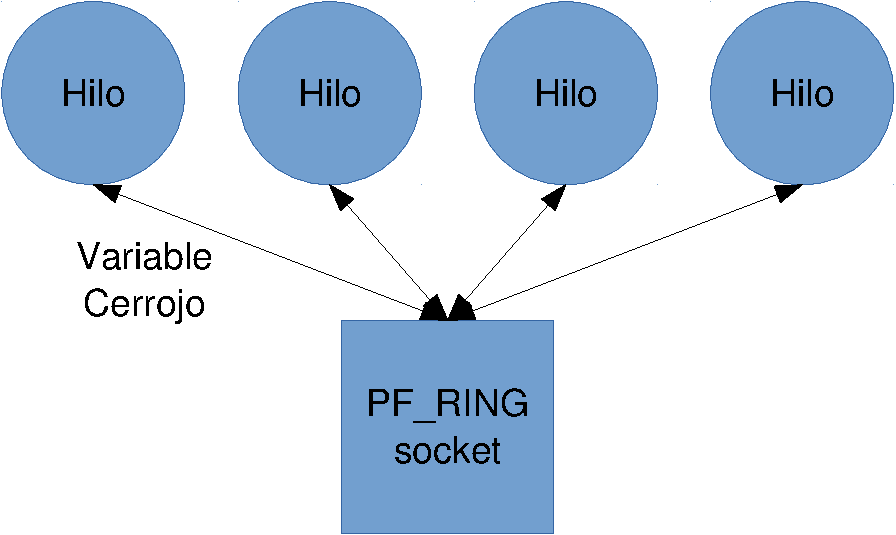
\includegraphics[width=\textwidth]{CapituloPF_RING/Figuras/CluserNoCluster-crop}%
    \LABFIG{PFRINGClusterNoCluster}
    \end{minipage}}
\hfill
\subfloat[Con Clustering]%
 {\begin{minipage}[t]{0.45\textwidth}
 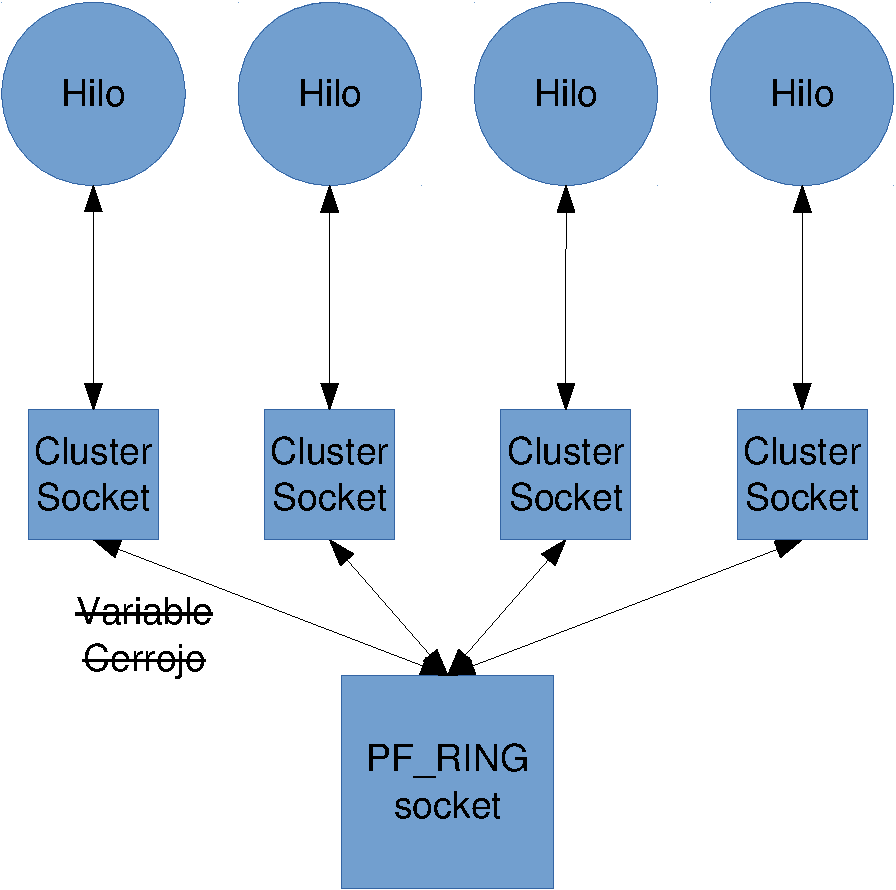
\includegraphics[width=\textwidth]{CapituloPF_RING/Figuras/CluserCluster-crop}%
 \LABFIG{PFRINGClusterCluster}
  \end{minipage}}
\caption{Ventajas de usar \texttt{PF\_RING} clustering}
\end{figure}
%

Un cluster \texttt{PF\_RING} persigue eliminar esa necesidad. En ligar de competir por los mismos recursos (el anillo 
\texttt{PF\_RING}), cada hilo tiene su propio socket, y el cluster se encarga de distribuir los paquetes a medida que 
éstos llegan. De esa forma, no es necesario bloquear los hilos cada vez que se desea leer un paquete, y todo el 
inter-bloqueo se realiza a nivel de núcleo, donde estas operaciones se hacen mucho más rápidas. Podemos ver una 
representación gráficas en las figuras \FIG{PFRINGClusterNoCluster} frente a \FIG{PFRINGClusterCluster} 
\cite{MonitoringUsingNtop}.

% \subsection{Ejemplo de ZeroCopy}
% Para probar la tecnología \texttt{PF\_RING ZeroCopy}, la distribución viene con algunos ejemplos\footnote{Se puede 
% descargar de forma gratuita desde 
% \url{https://svn.ntop.org/svn/ntop/trunk/PF_RING/userland/examples_zc/README.examples}} como un contador de paquetes 
% (\texttt{zcount}), un distribuidor basado en el clustering expuesto en la sección \SSEC{PacketClustering} 
% (\texttt{zbalance}), o una aplicación que es capaz de multiplexar varias interfaces en una sola (\texttt{zfifo}).
% 
% Si probamos, por ejemplo, la aplicación \texttt{zbalance} en una interfaz a la que estamos enviando paquetes a 1Gbps, y 
% no usamos \texttt{ZeroCopy}, observamos que somos capaces de alcanzar

\endinput

\begin{Resumen}[Resumen de PF RING]


\subsection*{S1}

\end{Resumen}

